\subsection*{Chen-Notation}
\usetikzlibrary{er}
\tikzset{multi attribute/.style={attribute,double distance=1.5pt}}
\tikzset{derived attribute/.style={attribute,dashed}}
\tikzset{total/.style={double distance=1.5pt}}

\newcommand{\key}[1]{\underline{#1}}

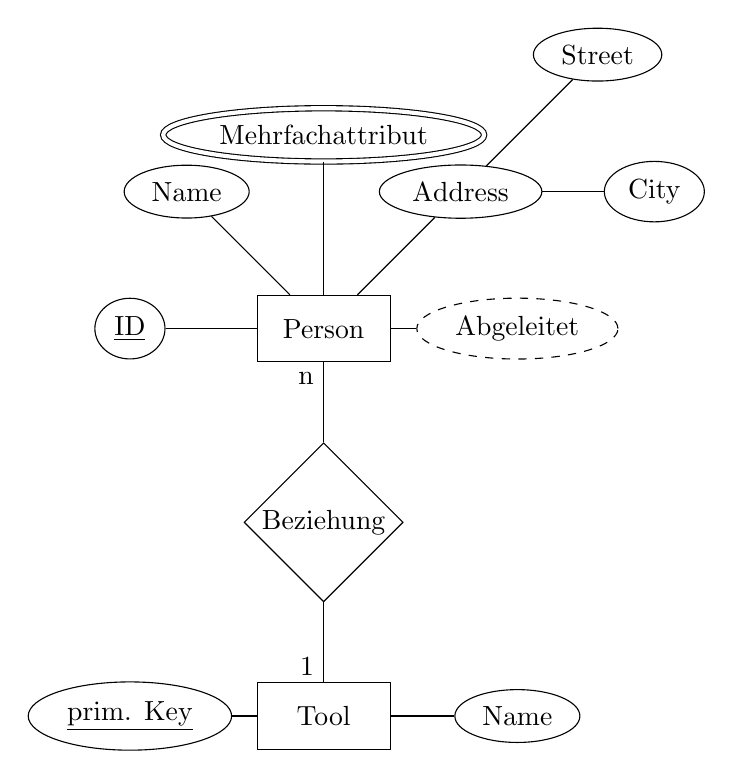
\begin{tikzpicture}[node distance=7em]
\node[entity](person){Person};
\node[attribute](pid)[left of=person]{\key{ID}}edge(person);
\node[attribute](name)[above left of=person]{Name}edge(person);
\node[multi attribute](phone)[above of=person]{Mehrfachattribut}edge(person);
\node[attribute](address)[above right of=person]{Address}edge(person);
\node[attribute](street)[above right of=address]{Street}edge(address);
\node[attribute](city)[right of=address]{City}edge(address);
\node[derived attribute](age)[right of=person]{Abgeleitet}edge(person);
\node[relationship](uses)[below of=person]{Beziehung}edge(person);
\node[entity](tool)[below of=uses]{Tool}edge(uses);
\node[attribute](tid)[left of=tool]{\key{prim. Key}}edge(tool);
\node[attribute](tname)[right of=tool]{Name}edge(tool);
\draw(tool) -- (uses) node[pos=0.2,left] {1};
\draw(uses) -- (person) node[pos=0.8,left] {n};
\end{tikzpicture}

\def\pk#1{\node[name=\entityname-#1, every property/.try]{#1};\node[name=\entityname-#1, every property/.try, red, text width=1in, align=right]{(PK)};\\}
\def\fk#1{\node[name=\entityname-#1, every property/.try]{#1};\node[name=\entityname-#1, every property/.try, red, text width=1in, align=right]{(FK)};\\}


\subsection*{Krähenfuß}
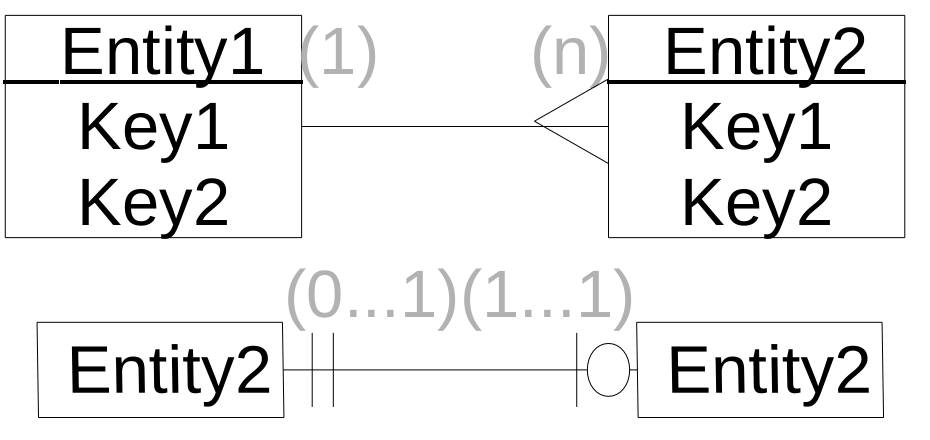
\includegraphics[width=0.2\textwidth]{crow}
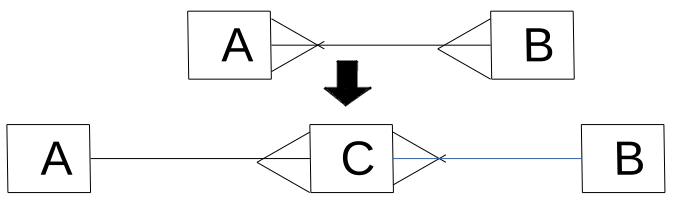
\includegraphics[width=0.2\textwidth]{m-n}